% Created by tikzDevice version 0.12.3.1 on 2022-10-30 20:05:30
% !TEX encoding = UTF-8 Unicode
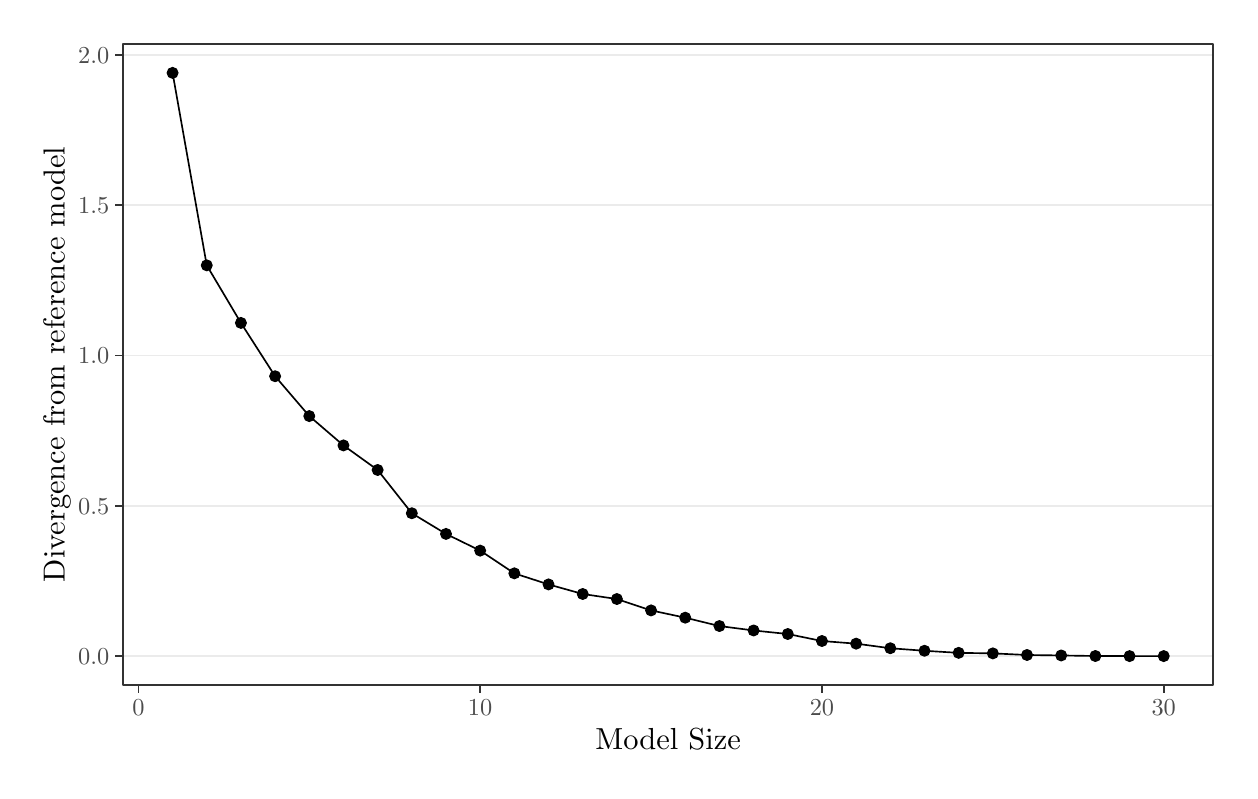
\begin{tikzpicture}[x=1pt,y=1pt]
\definecolor{fillColor}{RGB}{255,255,255}
\begin{scope}
\definecolor{drawColor}{RGB}{255,255,255}
\definecolor{fillColor}{RGB}{255,255,255}

\path[draw=drawColor,line width= 0.6pt,line join=round,line cap=round,fill=fillColor] (  0.00,  0.00) rectangle (433.62,268.00);
\end{scope}
\begin{scope}
\definecolor{fillColor}{RGB}{255,255,255}

\path[fill=fillColor] ( 34.16, 30.69) rectangle (428.12,262.50);
\definecolor{drawColor}{gray}{0.92}

\path[draw=drawColor,line width= 0.6pt,line join=round] ( 34.16, 41.22) --
	(428.12, 41.22);

\path[draw=drawColor,line width= 0.6pt,line join=round] ( 34.16, 95.54) --
	(428.12, 95.54);

\path[draw=drawColor,line width= 0.6pt,line join=round] ( 34.16,149.86) --
	(428.12,149.86);

\path[draw=drawColor,line width= 0.6pt,line join=round] ( 34.16,204.18) --
	(428.12,204.18);

\path[draw=drawColor,line width= 0.6pt,line join=round] ( 34.16,258.50) --
	(428.12,258.50);
\definecolor{drawColor}{RGB}{0,0,0}
\definecolor{fillColor}{RGB}{0,0,0}

\path[draw=drawColor,line width= 0.4pt,line join=round,line cap=round,fill=fillColor] ( 52.06,251.96) circle (  1.96);

\path[draw=drawColor,line width= 0.4pt,line join=round,line cap=round,fill=fillColor] ( 64.41,182.42) circle (  1.96);

\path[draw=drawColor,line width= 0.4pt,line join=round,line cap=round,fill=fillColor] ( 76.76,161.61) circle (  1.96);

\path[draw=drawColor,line width= 0.4pt,line join=round,line cap=round,fill=fillColor] ( 89.11,142.35) circle (  1.96);

\path[draw=drawColor,line width= 0.4pt,line join=round,line cap=round,fill=fillColor] (101.46,127.95) circle (  1.96);

\path[draw=drawColor,line width= 0.4pt,line join=round,line cap=round,fill=fillColor] (113.81,117.35) circle (  1.96);

\path[draw=drawColor,line width= 0.4pt,line join=round,line cap=round,fill=fillColor] (126.16,108.47) circle (  1.96);

\path[draw=drawColor,line width= 0.4pt,line join=round,line cap=round,fill=fillColor] (138.51, 92.84) circle (  1.96);

\path[draw=drawColor,line width= 0.4pt,line join=round,line cap=round,fill=fillColor] (150.86, 85.37) circle (  1.96);

\path[draw=drawColor,line width= 0.4pt,line join=round,line cap=round,fill=fillColor] (163.21, 79.33) circle (  1.96);

\path[draw=drawColor,line width= 0.4pt,line join=round,line cap=round,fill=fillColor] (175.56, 71.12) circle (  1.96);

\path[draw=drawColor,line width= 0.4pt,line join=round,line cap=round,fill=fillColor] (187.91, 67.12) circle (  1.96);

\path[draw=drawColor,line width= 0.4pt,line join=round,line cap=round,fill=fillColor] (200.26, 63.66) circle (  1.96);

\path[draw=drawColor,line width= 0.4pt,line join=round,line cap=round,fill=fillColor] (212.61, 61.84) circle (  1.96);

\path[draw=drawColor,line width= 0.4pt,line join=round,line cap=round,fill=fillColor] (224.96, 57.73) circle (  1.96);

\path[draw=drawColor,line width= 0.4pt,line join=round,line cap=round,fill=fillColor] (237.31, 55.10) circle (  1.96);

\path[draw=drawColor,line width= 0.4pt,line join=round,line cap=round,fill=fillColor] (249.66, 52.08) circle (  1.96);

\path[draw=drawColor,line width= 0.4pt,line join=round,line cap=round,fill=fillColor] (262.01, 50.48) circle (  1.96);

\path[draw=drawColor,line width= 0.4pt,line join=round,line cap=round,fill=fillColor] (274.36, 49.20) circle (  1.96);

\path[draw=drawColor,line width= 0.4pt,line join=round,line cap=round,fill=fillColor] (286.71, 46.67) circle (  1.96);

\path[draw=drawColor,line width= 0.4pt,line join=round,line cap=round,fill=fillColor] (299.06, 45.71) circle (  1.96);

\path[draw=drawColor,line width= 0.4pt,line join=round,line cap=round,fill=fillColor] (311.41, 44.06) circle (  1.96);

\path[draw=drawColor,line width= 0.4pt,line join=round,line cap=round,fill=fillColor] (323.76, 43.14) circle (  1.96);

\path[draw=drawColor,line width= 0.4pt,line join=round,line cap=round,fill=fillColor] (336.11, 42.39) circle (  1.96);

\path[draw=drawColor,line width= 0.4pt,line join=round,line cap=round,fill=fillColor] (348.46, 42.20) circle (  1.96);

\path[draw=drawColor,line width= 0.4pt,line join=round,line cap=round,fill=fillColor] (360.81, 41.62) circle (  1.96);

\path[draw=drawColor,line width= 0.4pt,line join=round,line cap=round,fill=fillColor] (373.16, 41.45) circle (  1.96);

\path[draw=drawColor,line width= 0.4pt,line join=round,line cap=round,fill=fillColor] (385.51, 41.25) circle (  1.96);

\path[draw=drawColor,line width= 0.4pt,line join=round,line cap=round,fill=fillColor] (397.86, 41.22) circle (  1.96);

\path[draw=drawColor,line width= 0.4pt,line join=round,line cap=round,fill=fillColor] (410.21, 41.22) circle (  1.96);

\path[draw=drawColor,line width= 0.6pt,line join=round] ( 52.06,251.96) --
	( 64.41,182.42) --
	( 76.76,161.61) --
	( 89.11,142.35) --
	(101.46,127.95) --
	(113.81,117.35) --
	(126.16,108.47) --
	(138.51, 92.84) --
	(150.86, 85.37) --
	(163.21, 79.33) --
	(175.56, 71.12) --
	(187.91, 67.12) --
	(200.26, 63.66) --
	(212.61, 61.84) --
	(224.96, 57.73) --
	(237.31, 55.10) --
	(249.66, 52.08) --
	(262.01, 50.48) --
	(274.36, 49.20) --
	(286.71, 46.67) --
	(299.06, 45.71) --
	(311.41, 44.06) --
	(323.76, 43.14) --
	(336.11, 42.39) --
	(348.46, 42.20) --
	(360.81, 41.62) --
	(373.16, 41.45) --
	(385.51, 41.25) --
	(397.86, 41.22) --
	(410.21, 41.22);
\definecolor{drawColor}{gray}{0.20}

\path[draw=drawColor,line width= 0.6pt,line join=round,line cap=round] ( 34.16, 30.69) rectangle (428.12,262.50);
\end{scope}
\begin{scope}
\definecolor{drawColor}{gray}{0.30}

\node[text=drawColor,anchor=base east,inner sep=0pt, outer sep=0pt, scale=  0.88] at ( 29.21, 38.19) {0.0};

\node[text=drawColor,anchor=base east,inner sep=0pt, outer sep=0pt, scale=  0.88] at ( 29.21, 92.51) {0.5};

\node[text=drawColor,anchor=base east,inner sep=0pt, outer sep=0pt, scale=  0.88] at ( 29.21,146.83) {1.0};

\node[text=drawColor,anchor=base east,inner sep=0pt, outer sep=0pt, scale=  0.88] at ( 29.21,201.15) {1.5};

\node[text=drawColor,anchor=base east,inner sep=0pt, outer sep=0pt, scale=  0.88] at ( 29.21,255.47) {2.0};
\end{scope}
\begin{scope}
\definecolor{drawColor}{gray}{0.20}

\path[draw=drawColor,line width= 0.6pt,line join=round] ( 31.41, 41.22) --
	( 34.16, 41.22);

\path[draw=drawColor,line width= 0.6pt,line join=round] ( 31.41, 95.54) --
	( 34.16, 95.54);

\path[draw=drawColor,line width= 0.6pt,line join=round] ( 31.41,149.86) --
	( 34.16,149.86);

\path[draw=drawColor,line width= 0.6pt,line join=round] ( 31.41,204.18) --
	( 34.16,204.18);

\path[draw=drawColor,line width= 0.6pt,line join=round] ( 31.41,258.50) --
	( 34.16,258.50);
\end{scope}
\begin{scope}
\definecolor{drawColor}{gray}{0.20}

\path[draw=drawColor,line width= 0.6pt,line join=round] ( 39.71, 27.94) --
	( 39.71, 30.69);

\path[draw=drawColor,line width= 0.6pt,line join=round] (163.21, 27.94) --
	(163.21, 30.69);

\path[draw=drawColor,line width= 0.6pt,line join=round] (286.71, 27.94) --
	(286.71, 30.69);

\path[draw=drawColor,line width= 0.6pt,line join=round] (410.21, 27.94) --
	(410.21, 30.69);
\end{scope}
\begin{scope}
\definecolor{drawColor}{gray}{0.30}

\node[text=drawColor,anchor=base,inner sep=0pt, outer sep=0pt, scale=  0.88] at ( 39.71, 19.68) {0};

\node[text=drawColor,anchor=base,inner sep=0pt, outer sep=0pt, scale=  0.88] at (163.21, 19.68) {10};

\node[text=drawColor,anchor=base,inner sep=0pt, outer sep=0pt, scale=  0.88] at (286.71, 19.68) {20};

\node[text=drawColor,anchor=base,inner sep=0pt, outer sep=0pt, scale=  0.88] at (410.21, 19.68) {30};
\end{scope}
\begin{scope}
\definecolor{drawColor}{RGB}{0,0,0}

\node[text=drawColor,anchor=base,inner sep=0pt, outer sep=0pt, scale=  1.10] at (231.14,  7.64) {Model Size};
\end{scope}
\begin{scope}
\definecolor{drawColor}{RGB}{0,0,0}

\node[text=drawColor,rotate= 90.00,anchor=base,inner sep=0pt, outer sep=0pt, scale=  1.10] at ( 13.08,146.59) {Divergence from reference model};
\end{scope}
\end{tikzpicture}
